\section{Resultados}

Uno de los métodos más usados para conseguir la alta disponibilidad en nuestro servidor Postgres es implementar la Replicación. Con ello nos aseguramos que nuestro sistema esté activo el 99,9\% del año.

A continuación se muestra el resultado obtenido al realizar la replicación. En la Figura \ref{fig:prueba1}. Se presenta la conexión a la base de datos "prueba", luego se crea una tabla llamada pruebillap y finalmente se ingresa un registro a la tabla creada anteriormente. 

\begin{figure}[H]
\centering
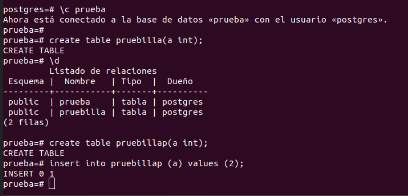
\includegraphics[width=\columnwidth]{gResult/prueba1}
\caption{Resultad.o}\label{fig:prueba1}
\end{figure}

Al generar una conexión con la maquina esclavo e ingresar a la base de datos prueba, se puede observar la actualización de la información al instante que es ingresada por el maestro, esto indica que la configuración fue exitosa. 





